\chapter{Segmentation interactive }

\section{Introduction}

Ce chapitre traite de la segmentation interactive. Comme son nom l'indique, ce domaine de recherche est rattaché à celui de la segmentation. Il comprend un ensemble de méthodes semi-automatiques, où l'utilisateur fournit les indications nécessaires à l'obtention d'un résultat. 

Afin de bien en comprendre les enjeux, nous commencerons par quelques rappels sur la \modif{segmentation qui} nous permettront de définir la segmentation interactive. Nous nous intéresserons ensuite aux différentes pistes explorées jusqu'à présent et nous présenterons quelques algorithmes clés de l'état de l'art. 


\subsection{Segmentation}

La segmentation est une étape \modif{clé pour} un grand nombre de \modif{méthodes} d'analyse d'images. Son but consiste à produire une partition des pixels de l'image en composantes connexes, selon des critères prédéfinis (homogénéité en \modif{termes} de couleurs, de texture, etc.). Ces composantes connexes sont nommées régions et correspondent à des objets ou à des parties d'objets, formant un pavage de l'image en primitives visuelles de haut niveau. La figure \ref{fig:sota:seg-ex} contient un exemple de segmentation. Les pixels de l'image originale (figure \ref{fig:sota:seg-ex}a) sont groupés en une dizaine de régions (figure \ref{fig:sota:seg-ex}b). La figure \ref{fig:sota:seg-ex}c représente les contours de ces régions, \modif{où apparaissent} en blanc les pixels ayant un de leurs voisins qui appartient à une autre région.

\begin{figure}[htb]
\centering
	 \begin{subfigure}[t]{0.3\textwidth}	
			\includegraphics[width=\textwidth]{images/etat-de-l-art/img-065-im}
		 \caption{Image originale. }
	\end{subfigure}
	~
	 \begin{subfigure}[t]{0.3\textwidth}	
			\includegraphics[width=\textwidth]{images/etat-de-l-art/img-065-seg}
		 \caption{Segmentation \modif{de} cette image : une couleur par \modif{région.}}
	\end{subfigure}
	~
	 \begin{subfigure}[t]{0.3\textwidth}	
			\includegraphics[width=\textwidth]{images/etat-de-l-art/img-065-bdr}
		 \caption{Contours des régions de cette segmentation.}
	\end{subfigure}
	\caption{Exemple \modif{de} segmentation.}
	\label{fig:sota:seg-ex}
\end{figure}


Trois \modif{hypothèses} guident les travaux menés en segmentation :
\begin{itemize}
\item l'homogénéité à l'intérieur de chaque région en \modif{termes} de couleur \modif{ou} de texture doit être maximisée ;
\item les similitudes entre les différentes régions doivent être minimisées ;
\item les pixels voisins appartenant à des régions différentes doivent être aussi dissemblables que possible.
\end{itemize} 



\subsection{Segmentation sémantique}

Tandis que la segmentation se contente de produire un pavage de l'image en régions, la segmentation sémantique réalise une partition des pixels en ensembles qui correspondent \modif{à des catégories d'objets}. Comme un même objet peut correspondre à plusieurs régions \modif{ou plusieurs objets de la même catégorie être présents dans l'image}, les ensembles ne sont pas nécessairement des composantes connexes. Si le problème de la segmentation peut être vu comme la recherche des frontières des objets présents dans une photographie, celui de la segmentation sémantique consiste à  localiser et identifier les \modif{objets qui la composent c'est-à-dire comme la résolution d'un problème de classification, avec une classe par catégorie d’objets}. La figure \ref{fig:sota:seg-sem-ex}b contient \modif{une} segmentation sémantique associée à la figure \ref{fig:sota:seg-sem-ex}a. Les pixels se répartissent en trois ensembles : le premier correspondant à une table en bois (en jaune), le second à la chenille (en rose) et le troisième à la branche de tomate (en bleu).

\begin{figure}[htb]
\centering
	 \begin{subfigure}[t]{0.3\textwidth}	
			\includegraphics[width=\textwidth]{images/etat-de-l-art/img-065-im}
		 \caption{Image originale. }
	\end{subfigure}
	~
	 \begin{subfigure}[t]{0.3\textwidth}	
			\includegraphics[width=\textwidth]{images/etat-de-l-art/img-065-seg-semantique}
		 \caption{Segmentation sémantique \modif{de} cette image. Trois classes sont \modif{identifiées} : le bois (en jaune), la chenille (en rose) et la tomate (en bleu).}
	\end{subfigure}
	\caption{\modif{Exemple de} segmentation sémantique.}
	\label{fig:sota:seg-sem-ex}
\end{figure}


L'utilisation des réseaux de neurones convolutifs (CNN, de l'anglais \og \emph{Convolutional Neural Networks} \fg) \modif{et de l'apprentissage profond ont} conduit à des \modif{avancées} significatives dans le domaine la \modif{segmentation} sémantique  \cite{fourure2017multi,garcia2017review,long2015fully}. Toutefois, malgré la qualité impressionnante des \modif{résultats} obtenus,  ce type de méthode ne peut être guidée que lors de l'étape d'apprentissage \cite{lin2016scribblesup}. 

L'un des inconvénients les plus évidents de cette contrainte réside dans le fait que lorsque la méthode produit une segmentation erronée, il n'est pas possible de \modif{la} corriger sans recommencer l'apprentissage du CNN, lequel nécessite \modif{une quantité de données d'apprentissage importante et} de nombreuses heures de calculs. \modif{Par ailleurs, le CNN est entraîné à reconnaître un nombre fini de classes, définies lors de l'apprentissage. Pour introduire une nouvelle classe, il faut recommencer l'étape d'apprentissage.} 

La résolution de ces deux problèmes \modif{peut passer} par la recherche de méthodes semi-au\-to\-ma\-ti\-ques, intégrant de manière plus souple l'intervention d'un utilisateur. Elle correspond au domaine de la segmentation \modif{interactive}. 

\subsection{Segmentation interactive }

Le principe de la segmentation interactive consiste guider la recherche d'une segmentation particulière en intégrant quelques indications fournies par un utilisateur. Le fonctionnement général d'une méthode de segmentation interactive est illustré par la figure \ref{fig:sota:segInt}. Une photographie est donnée à l'utilisateur qui décide des \modif{entités} qu'il souhaite \modif{sélectionner}. \modif{Notons que l'utilisateur peut choisir ou non de produire une segmentation sémantique. Dans certains cas, il souhaitera sélectionner ensemble tous les objets d'une même catégorie (par exemples, tous les arbres). Dans d'autres, il pourra ne vouloir sélectionner qu'un seul objet, appartenant à une catégorie représentée plusieurs fois dans l'image (par exemple, un arbre spécifique).}

Les indications \modif{que l'utilisateur} donne permettent à la méthode de produire un premier résultat. Le plus souvent ce dernier ne correspond pas exactement aux attentes de l'utilisateur, qui vient ajouter ou supprimer des indications, déclenchant la recherche d'une deuxième segmentation. Ce processus est répété jusqu'à satisfaction des objectifs de l'utilisateur.

\begin{figure}[htb]
	\centering
		\includegraphics[width=0.45\textwidth]{images/etat-de-l-art/segInt}
		\caption{Processus\modif{, pouvant être itératif}, d'utilisation d'une méthode de segmentation interactive.}
		 \label{fig:sota:segInt}
\end{figure}


\modif{Soit $I$ une image}.  Soit \modif{$\mathbb{P}=\lbrace p_{1}, \cdots, p_{N_{I}} \rbrace$} l'ensemble des $N_{I}$ pixels de $I$. Soit \modif{$\Lambda=\lbrace \lambda_{1},\cdots,\lambda_{N_{\Lambda}} \rbrace$} un ensemble de $N_{\Lambda}$ labels indexant chaque classe, avec une classe par \modif{entité} \modif{que l'utilisateur souhaite sélectionner}.  Les indications données par l'utilisateur prennent la forme d'un ensemble  $G= \lbrace g_{1}, \cdots, g_{N_{G}} \rbrace$ dont chaque élément $g_{i}$ est un couple de valeurs $(p_{i},\lambda_{j})$, tel que  \modif{$p_{i} \in \mathbb{P} $} et \modif{$\lambda_{i} \in \Lambda$}. Réaliser une segmentation interactive de $I$ consiste à associer à chaque élément de \modif{$\mathbb{P}$} un unique élément de \modif{$\Lambda$}, en garantissant le maximum de cohérence :
\begin{itemize}
\item avec le contenu de l'image ;
\item entre les pixels attribués à une classe et les indications données par l'utilisateur.
\end{itemize}

La communication de l'utilisateur vers la méthode s'effectue par le biais des indications (l'ensemble $G$). \modif{Certaines méthodes de segmentation interactive considèrent ces indications comme parfaitement fiables \cite{boykov2001interactive,salembier2000binary}, d'autres comme pouvant contenir des erreurs \cite{ Changjae2017Robust,muller2016robust}}. La communication de la méthode vers l'utilisateur \modif{est assurée} par l'affichage d'une segmentation de l'image.

Ces deux caractéristiques imposent, entre autres : 
\begin{itemize}
\item que l'impact d'une indication sur le résultat soit facilement prévisible par l'utilisateur, afin qu'il puisse guider efficacement la méthode ;
\item que les modalités d'\modif{interaction} permettant d'ajouter ou de retirer une indication soient faciles d'utilisation ;
\item que le temps nécessaire pour obtenir une segmentation à partir d'une image et d'un ensemble d'indications demeure suffisamment court pour permettre une interaction fluide (généralement nous considérerons que cette durée ne peut excéder quelques secondes).
\end{itemize}

Il s'avère intéressant de mettre ce dernier point en relation avec le contexte d'application des méthodes de segmentation interactive. Actuellement, ces dernières sont employées afin de sélectionner des objets au sein d'une photographie pour leur appliquer des traitements particuliers ou pour les intégrer au sein d'un collage, dans le domaine artistique ou dans celui du design. Les images à traiter comportent souvent plusieurs millions de pixels, ce qui soulève la question du passage à l'échelle des algorithmes de segmentation interactive. Enfin, si actuellement la majorité de ces méthodes sont implémentées pour des ordinateurs, le remplacement progressif de ce type de machine par des smartphones auprès du grand \modif{public} requiert d'envisager des algorithmes capables de passer à l'échelle malgré des contraintes matérielles \modif{importantes} (taille de la mémoire vive, capacité du processeur, puissance de la carte graphique, etc.).


\subsection{Catégorisation}

\modif{Durant ces} deux dernières décennies, le domaine de la segmentation interactive s'est enrichi de nombreux algorithmes.  Dans ce mémoire, nous proposons de les classer en trois catégories :
\begin{itemize}
\item \textbf{Binarisation interactive par recherche des contours - } Ces algorithmes déterminent pour chaque pixel s'il appartient ou non au contour de l'objet d'intérêt. Il s'agit donc d'un problème de classification à deux classes,  $\lambda_{C}$ pour les pixels du contour, $\lambda_{\neg C}$ pour les autres.  L'utilisateur indique quelques pixels de la classe $\lambda_{C}$. 
\item \textbf{Binarisation interactive par recherche des régions - } Ces algorithmes groupent les pixels de manière à obtenir deux ensembles homogènes. Ces ensembles \modif{correspondent} à une ou plusieurs composantes connexes. Il s'agit là aussi d'un problème de classification à deux classes avec, d'une part, les pixels de l'objet principal ($\lambda_{O}$) et, d'autre part, ceux du fond  ($\lambda_{F}$). L'utilisateur attribue quelques pixels à chacune des deux classes. 
\item \textbf{Segmentation interactive \modif{multiclasse} - } Ces algorithmes correspondent à une généralisation de la catégorie précédente, où le nombre de classes n'est plus limité à deux. 
\end{itemize}



\section{\modif{Lexique et notations}}

\subsection{\modif{Lexique}}
Par la suite, nous utiliserons \modif{les termes} :

\begin{itemize}
\item \textbf{germe}, pour désigner le pixel attribué à une classe par l'utilisateur (un germe correspond à une indication)  ;
\item \textbf{classe},  pour désigner  une \modif{entité (un objet ou une catégorie d'objets)} à laquelle certains pixels seront assignés à l'issue du processus de segmentation;
\item \textbf{segmentation}, pour désigner le résultat produit par une méthode de segmentation interactive à chaque itération ;
\item \textbf{région}, pour désigner un ensemble de pixels connexes appartenant à la même classe.
\end{itemize}

\subsection{Notations}

Soit $I$ une image.
\begin{itemize}
\item \textbf{L'ensemble} $\mathbb{P}= \lbrace p_{1}, \cdots, p_{N_{I}} \rbrace$ contient les pixels de $I$.
\item \textbf{La fonction}  $\nei(p)$ donne l'ensemble des pixels voisins du pixel $p$.  La figure \ref{fig:sota:vois} décrit les trois principaux systèmes de voisinage : les quatre voisins (nord, est, sud, ouest), les huit voisins (nord, nord-est, est, sud-est, sud, sud-ouest, ouest, nord-ouest) et le voisinage circulaire qui comprend les $N_{voi}$ voisins répartis \modif{régulièrement} sur le cercle \modif{de rayon $r$} ayant pour centre le pixel $p$. Dans ce dernier cas, le niveau de gris d'un voisin est obtenu par interpolation des niveaux de gris environnants.
\begin{figure}[htb]
	\centering
	 \begin{subfigure}[t]{0.2\textwidth}	
			\includegraphics[width=\textwidth]{images/etat-de-l-art/4V}
		 \caption{4-voisinage.}
			\label{fig:sota:vois4}
	\end{subfigure}
	~
	 \begin{subfigure}[t]{0.2\textwidth}	
			\includegraphics[width=\textwidth]{images/etat-de-l-art/8V}
		 \caption{8-voisinage.}
			\label{fig:sota::vois8}
	\end{subfigure}
	~
	 \begin{subfigure}[t]{0.2\textwidth}	
			\includegraphics[width=\textwidth]{images/etat-de-l-art/CV}
		 \caption{Voisinage circulaire.}
			\label{fig:sota::voisC}
			
	\end{subfigure}
	\caption{Les principaux systèmes de voisinage pour un pixel.}
	\label{fig:sota:vois}
\end{figure}

\item \textbf{Le graphe} $\mathcal{G}=\ <V,E>$ est une représentation de $I$, où $V=\lbrace v_{1},\cdots, v_{N_{I}} \rbrace$ est un ensemble de $N_{I}$ sommets correspondant aux pixels de $I$ et $E$ un ensemble d'arêtes reliant les sommets $v_{i}$ et $v_{j}$ si et seulement s'ils correspondent à des pixels voisins. Un exemple d'un tel graphe est donné sur la figure \ref{fig:sota:im_to_g}.

\item \textbf{L'arête} $e_{i,j}$ relie les sommets $v_{i}$ et $v_{j}$, correspondant respectivement aux   \modif{$i\ieme$}  et  \modif{$j\ieme$}  pixels. 
\item \textbf{Le poids }$w_{i,j}$ est le réel associé à l'arête $e_{i,j}$.
\item \textbf{Une segmentation } \modif{$S = \lbrace s_{1}, \cdots, s_{N_{S}} \rbrace$} de $I$ consiste en  une partition de $\mathcal{G}$ en $N_{S}$ \modif{composantes connexes}.
\item \textbf{L'ensemble} \modif{$ \Lambda =\lbrace \lambda_{1},\cdots,\lambda_{N_{\Lambda}}  \rbrace $} contient les labels associés aux $N_{\Lambda}$ classes.
\item \textbf{Les germes donnés par l'utilisateur} sont représentés sous la forme d'un ensemble $G= \lbrace g_{1}, \cdots, g_{N_{G}} \rbrace$, où chaque élément $g_{i}$ est un couple de valeurs $(p_{i},\lambda_{j})$, tel que \modif{$p_{i} \in \mathbb{P}$}  \modif{et $\lambda_{i} \in \Lambda$}.
\item \textbf{La fonction de coût} $ \mathcal{F}(I,S,G)$ permet d'évaluer la pertinence d'une segmentation $S$ de $I$, par rapport aux caractéristiques intrinsèques de $I$ et aux germes $G$.  
\end{itemize}


\begin{figure}[htb]
	\centering
	 \begin{subfigure}[t]{0.3\textwidth}	
			\includegraphics[width=\textwidth]{images/etat-de-l-art/grahIm}
		 \caption{Réprésentation d'une image couleur de $4 \times 4$ pixels.}
			\label{fig:sota:img_graph1}
	\end{subfigure}
	~
	 \begin{subfigure}[t]{0.3\textwidth}	
			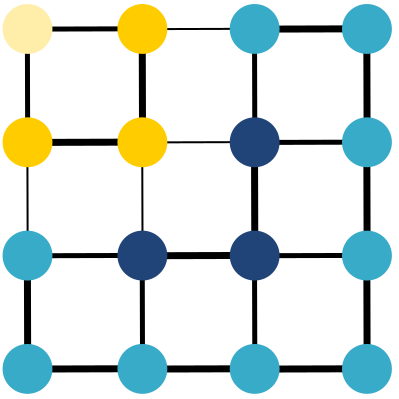
\includegraphics[width=\textwidth]{images/etat-de-l-art/grahIm2}
		 \caption{Graphe construit à partir de l'image. Nous considérons ici que les pixels
		 sont voisins au sens du 4-voisinage. L'épaisseur des arêtes est proportionnelle au degré de similarité entre les pixels.}
			\label{fig:sota::img_graph1}
	\end{subfigure}
	\caption{Représentation d'une image par un graphe.}
	\label{fig:sota:im_to_g}
\end{figure}

\section{Méthodes de binarisation interactive par recherche des contours}

\subsection{Formulation du problème}

Les méthodes de binarisation interactive par recherche des contours séparent un objet du fond en retrouvant les pixels correspondant à son contour. Il s'agit d'un problème de classification à deux classes,  $\lambda_{C}$ si le pixel appartient au contour,  $\lambda_{\neg C}$ sinon. Les germes sont quelques uns des pixels \modif{du contour}. L'ensemble $G$ correspond \modif{donc} à des pixels de label $\lambda_{C}$. 

Soit \modif{$\mathbb{P}_{C}$}, l'ensemble des pixels de label $\lambda_{C}$ \modif{dans le résultat donné par la méthode}. Cet ensemble doit respecter les propriétés suivantes :
\begin{itemize}
\item il doit contenir l'ensemble des pixels de $G$ ;
\item il doit avoir une forte probabilité d'appartenir aux contours de $I$ ;
\item il doit former une courbe fermée (voir la figure \ref{fig:sota:courbeSimp}) ;
\item cette courbe doit être aussi simple que possible et notamment éviter de se croiser (voir la figure \ref{fig:sota:courbeX}) ou de se chevaucher (voir la figure \ref{fig:sota:courbeChe}).
\end{itemize} 

\modif{Il n'existe pas à ce jour de méthode de binarisation interactive par recherche des contours résolvant} des problèmes multiclasses : le chemin formé par les pixels de label  $\lambda_{C}$ étant fermé, la segmentation $S$ obtenue \modif{contient uniquement deux régions}, l'une correspondant à l'objet à extraire $S_{O}$ et l'autre au fond $S_{F}$.  

\begin{figure}[htb]
	\centering
	 \begin{subfigure}[t]{0.25\textwidth}	
			\includegraphics[width=\textwidth]{images/etat-de-l-art/courbe3}
		 \caption{Courbe simple.}
			\label{fig:sota:courbeSimp}
	\end{subfigure}
	~
	 \begin{subfigure}[t]{0.25\textwidth}	
			\includegraphics[width=\textwidth]{images/etat-de-l-art/courbe2}
		 \caption{Courbe se croisant.}
			\label{fig:sota:courbeX}
	\end{subfigure}
	~
	 \begin{subfigure}[t]{0.25\textwidth}	
			
\includegraphics[width=\textwidth]{images/etat-de-l-art/courbe1}
		 \caption{Courbe se chevauchant. }
			\label{fig:sota:courbeChe}
	\end{subfigure}
	\caption{Quelques types de courbes.}
	\label{fig:sota:courbes}
\end{figure}

\subsection{Interaction avec l'utilisateur}

La figure \ref{fig:sota_boundary_based_ihm} illustre le type \modif{d'indications généralement associé} aux méthodes de binarisation par recherche des contours. Les germes donnés par l'utilisateur sont représentés par de petits disques clairs. Le contour trouvé par la méthode est affiché sur la forme de traits blancs bordés de noir. Lorsque celui-ci s'avère erroné, l'utilisateur peut ajouter, déplacer ou supprimer certains germes. 

\begin{figure}[htb]
	\centering
			\includegraphics[height=0.35\textheight]{images/etat-de-l-art/boundary-based-method2}
		 \caption{Binarisation interactive par recherche des contours : exemple d'interaction avec l'utilisateur. \modif{ Les germes donnés par l'utilisateur apparaissent sous la forme de disques blancs. Le contour trouvé par la méthode est indiqué par un trait blanc bordé de noir.}}
		 \label{fig:sota_boundary_based_ihm}
\end{figure}

Même s'il permet de modifier facilement la forme de la courbe, ce mode d'interaction présente deux désavantages. Tout d'abord, dans des zones où les contours n'apparaissent pas de manière nette (par exemple parce que l'objet est flou ou en raison d'un faible contraste), l'utilisateur peut être contraint de donner de très nombreux germes, ce qui rend rapidement le procédé fastidieux et frustrant. Ensuite, du fait qu'aucune erreur n'est tolérée dans les germes (ces derniers doivent être exactement sur le contour de l'objet), il demande à l'utilisateur de pouvoir les désigner avec précision. Si celle-ci est facilement obtenue à l'aide d'un périphérique tel qu'une souris ou une tablette graphique, elle devient problématique pour du matériel reposant sur un écran tactile, tel que les tablettes ou les smartphones. 

\subsection{Méthode de Mortensen \textit{et al.}}

\modif{Proposé} par Mortensen \textit{et al.}, l'algorithme des ciseaux intelligents \cite{mortensen1995intelligent} formule la détection du contour d'un objet (donc des pixels de label $\lambda_{C}$) comme un problème de recherche du plus court chemin au sein d'un graphe. Chaque arête $e_{i,j} \in E$ est pondérée à l'aide de la \modif{mesure suivante} : \modif{
\begin{equation}
 \mathcal{F} _{sim}(i,j) = \nombre{0,43}f_{1}(j) + \nombre{0,43}f_{2}(j) + \nombre{0,14}f_{3}(i,j) 
\end{equation}}
où
\begin{itemize}
\item la fonction binaire $f_{1}$ correspond à la réponse d'un détecteur de contour par passage à 0 du laplacien ;
\item $f_{2}$ \modif{renvoie une} valeur inversement proportionnelle à celle de la norme du gradient de $I$ ;
\item $f_{3}$ est une fonction de régularisation, favorisant les contours réguliers, en pénalisant les variations brusques de la direction du contour.
\end{itemize}

Soit $I_{Lap}$ le résultat de la convolution d'une image $I$ par le \modif{masque laplacien $K_{Lap}$ : }
\begin{equation}
K_{Lap} = 
\label{eq:sota:laplacien}
\begin{bmatrix}
0 & 1 & 0\\
1 & -4 & 1\\
0 & 1 & 0
\end{bmatrix}\text{.}
\end{equation}

La matrice $I_{Lap}$ correspond à une approximation \modif{du laplacien de $I$} \modif{dont les passages à 0 coïncident théoriquement avec des points de contour dans l'image}. Mortensen \textit{et al.} \modif{détectent  un élément $I_{Lap}(i)$ comme un point de contour} si au moins l'un de ses voisins est de signe différent et si \modif{sa} valeur absolue est inférieure ou égale à la valeur absolue de \modif{chacun de }ses voisins. \modif{Dans ce cas, $f_{1}$} retourne 0, sinon elle renvoie la valeur $1$.

Soit \modif{$I_{x}(j)$} (respectivement \modif{$I_{y}(j)$}) l'approximation discrète de la composante horizontale (respectivement verticale) du vecteur gradient de la fonction niveau de gris de l'image $I$ pour le \modif{$j\ieme$ pixel}. La norme du vecteur gradient de $I$ est obtenue en calculant :
\modif{
\begin{equation}
Grad(j) =\sqrt{\modif{{I_{x}^{2}(j)} + {I_{y}^{2}(j)}}}
\end{equation}
}
et
\modif{
\begin{equation}
f_{2}(j) = \frac{\max(Grad) -Grad(j) }{\max(Grad)}\text{.}
\end{equation}
}

Ainsi, les valeurs retournées par les fonctions $f_{1}$ et $f_{2}$ sont d'autant plus petites que le pixel a une forte probabilité d'appartenir à \modif{l'un} des contours de l'image.

La fonction $f_{3}$, quant à elle, pénalise les changements brusques au niveau de la courbe.

Soit \modif{
\begin{equation}
\overrightarrow{p}_{\perp} =  \frac{\begin{bmatrix}I_y&-I_x\end{bmatrix}^\top}{\|\begin{bmatrix}I_y&-I_x\end{bmatrix}^\top\|}
\end{equation}}
le vecteur unitaire perpendiculaire à la direction du gradient.  \modif{Soit $\overrightarrow{p_{i}}_{\perp}$ ce vecteur pour le $i\ieme$ pixel.} Soit $\overrightarrow{p_{i,j}}$ le vecteur unitaire pointant du \modif{$i\ieme$} pixel vers le  \modif{$j\ieme$} pixel.
Soit le lien bidirectionnel entre les pixels $p{_i}$ et $p_{j}$ : 
\begin{equation}
f_{d}(i,j) =  \begin{cases}
 \overrightarrow{p_{i,j}} &\text{ si }  \overrightarrow{p_{i}}_{\perp} \cdot \overrightarrow{p_{i,j}} \geqslant 0\\
 \overrightarrow{p_{j,i}} &\text{ sinon. }
\end{cases}
\end{equation}
Le terme de lissage de Mortensen \textit{et al.} est calculé de la manière suivante :
\modif{
\begin{equation}
f_{3}(i,j) = \dfrac{2}{3\pi}\bigg(\acos \left(\overrightarrow{p_{i}}_{\perp} \cdot f_{d}(i,j) \right) + \acos(f_{d}(i,j) \cdot \overrightarrow{p_{j}}_{\perp}) \bigg).
\end{equation}
}
Le poids de chaque fonction a été déterminé de manière empirique par Mortensen \textit{et al.} Chaque fois que l'utilisateur indique qu'un pixel appartient au contour de l'objet, le chemin le plus court entre ce pixel et le précédent pixel \modif{sélectionné} est calculé, grâce à l'algorithme de Dijkstra \cite{Dijkstra59anote}. \modif{La courbe est donc construite au fur et à mesure}.

 Mortensen \textit{et al.} proposent une variante de l'algorithme des ciseaux intelligents \cite{mortensen1998interactive}, avec une fonction de similarité plus complexe, dont les poids sont mis à jour à la volée, à partir des caractéristiques des pixels du contour précédemment détectés. Cette variante s'avère pertinente dans le cas où la différence entre l'objet à extraire et le fond est moins marquée que les différences entre certaines composantes au sein de l'une ou l'autre de ces deux classes. La figure \ref{fig:sota_CI_avec_app_ex} montre un exemple de ce cas de figure. L'objet à segmenter est le ventricule gauche, dont le contour est bien moins marqué que celui du cœur. 
 
\begin{figure}[htb]
	\centering
			\includegraphics[width=0.25\textwidth]{images/etat-de-l-art/CI_avec_app_ex}
		 \caption{Exemple d'image pour laquelle le contour de l'objet à extraire (en bleu) est moins marqué que le contour entre différents éléments du fond.}
		 \label{fig:sota_CI_avec_app_ex}
\end{figure}

Une autre solution apportée à ce même problème consiste à ne chercher le plus court chemin que dans une partie du graphe. Le plus souvent, \modif{cette} partie correspond à un rectangle englobant les points de départ et d'arrivé du chemin. 

\subsection{Méthode de Mille \textit{et al.}}

L'algorithme par combinaison de chemins géodésiques \cite{mille2015combination} est l'une des plus récentes contributions dans le domaine de la binarisation interactive par recherche des contours. Conçu par Mille \textit{et al.}, il repose sur la recherche d'un chemin fermé  $C$ minimisant
\modif{
\begin{equation}
\mathcal{F}_{CCG}(I,C) = f_{1}(C) + w_{2}f_{2}(I,C) + w_{3}f_{3}(I,C)
\end{equation}
}
avec :
\begin{itemize}
\item \modif{$f_{1}$} une fonction de lissage, dont le résultat est un réel positif qui augmente lorsque certaines portions de la courbe se chevauchent et lorsque la courbe contient des boucles ;
\item \modif{$f_{2}$} une fonction favorisant le passage de la courbe \modif{par} des pixels appartenant aux contours de l'image, en effectuant la somme de l'inverse des normes des vecteurs \modif{gradients} des points de la courbe  ;
\item \modif{$f_{3}$} une fonction qui, en utilisant les coefficients de Bhattacharyya, favorise la production de régions à l'intérieur et à l'extérieur de la \modif{courbe dont} les couleurs correspondent à des distributions statistiques différentes.
\end{itemize} 

À l'instar de l'algorithme des ciseaux intelligents, les germes donnés par l'utilisateur sont ordonnés et forment l'ensemble \modif{$G=\lbrace g_{0}, \cdots, g_{i}, g_{i+1}, \cdots, g_{N_{G}-1} \rbrace$}, où \modif{$g_{i-1}$ est le $i\ieme$ }germe donné par l'utilisateur. Tandis que l'algorithme de Mortensen \textit{et al.} repose sur une approche locale, se contentant de rechercher un chemin optimal entre chaque couple \modif{$(g_{i},g_{((i+1) \mod N_{G})})$}, la méthode de Milles \textit{et al.} \modif{prend en compte} la totalité de la courbe et recherche la \emph{combinaison de chemins} qui minimise $\mathcal{F}_{CCG}$. 


Un parcours exhaustif de l'ensemble de ces combinaisons n'étant pas possible, l'algorithme produit une approximation de la solution en réalisant une \modif{présélection} de chemins probables pour chaque couple \modif{$(g_{i},g_{((i+1) \mod N_{G})})$}. Soit $C_{i}^{*}=\lbrace c_{i}^{1}, \cdots, c_{i}^{m} \rbrace$ l'ensemble de ces chemins probables reliant $g_{i}$ à \modif{$g_{((i+1) \mod N_{G})}$}. \modif{Soit une fonction $f_{D}( c_{i}^{j})$ renvoyant une valeur d'autant moins élevée que le chemin passe par peu de pixels et que ces pixels ont une forte probabilité d'appartenir à un contour, une approximation de la probabilité d'appartenir à un contour étant calculée à partir de la norme du vecteur gradient de la fonction niveau de gris de l'image $I$. Le chemin $c_{i}^{1}$ est le  chemin entre  $g_{i}$ et$g_{((i+1) \mod N_{G})}$, pour lequel la valeur de  $f_{D}$ est minimale}. Le chemin suivant, $c_{i}^{2}$, est obtenu en recherchant à nouveau le plus court chemin, mais sous la contrainte que  $c_{i}^{1}$ et  $c_{i}^{2}$ soient parfaitement distincts, \modif{c'est-à-dire que leurs seuls pixels communs soient $g_{i}$ et $g_{((i+1) \mod N_{G})}$}. 

Même en se limitant à un ensemble discret de chemins possibles entre chaque paire de germes consécutifs, une recherche directe de la combinaison minimisant $\mathcal{F}_{CCG}$ se révèle trop coûteuse en \modif{termes} de temps de calcul. Milles \textit{et al.} \modif{proposent} une heuristique où les chemins entre deux germes sont ordonnés en fonction de leur aire signée, calculée à l'aide du théorème de Green. \modif{Si nous considérons la droite $D_{i}$ passant par deux germes \modif{$g_{i}$ et $g_{((i+1) \mod N_{G})}$} ainsi que la surface $S_{i}^{j}$ délimitée par cette dernière et un chemin donné $c_{i}^{j}$, l'aire signée est calculée en soustrayant l'aire des parties de $S_{i}^{j}$ situées au dessous de $D_{i}$  à l'aire des parties de $S_{i}^{j}$ situées au dessus}.  L'algorithme est initialisé avec les chemins ayant la plus faible aire signée. À chaque itération, une série de combinaisons est produite à partir de la combinaison précédente, en ne changeant qu'un seul chemin. La combinaison minimisant $\mathcal{F}_{CCG}$ est sélectionnée et le processus répété jusqu'à convergence.  

\section{Méthodes de binarisation interactive par recherche des régions}

\subsection{Formulation du problème}
Les algorithmes de binarisation interactive orientés régions cherchent à produire une classification des pixels de l'image en deux catégories : l'objet à extraire (associé au label $\lambda_{O}$) et le fond (associé au label $\lambda_{F}$).  L'utilisateur guide la méthode en associant quelques pixels à chacune des deux classes. Il existe donc une partition de $G$ en deux sous-ensembles, $G_{O}$ pour les germes de label $\lambda_{O}$ et $G_{F}$ pour ceux de label $\lambda_{F}$. 

La segmentation produite par ce type d'algorithme correspond à une partition de l'image en $N_{R}$ régions, $N_{R}$ pouvant être supérieur à deux. Les solutions proposées pour ce problème s'articulent autour de deux grands types d'approches : la minimisation d'une \modif{fonction de coût} et la fusion de régions. 

\subsubsection{Minimisation \modif{d'une fonction de coût}}
Les algorithmes par minimisation \modif{d'une fonction de coût} reposent sur la définition d'une  fonction  de la forme : 
\modif{
\begin{equation}
\mathcal{F}_{C}(I,S,G) = \mathcal{F}_{D}(I,S,G) + \mathcal{F}_{R}(S)
\end{equation}
}
avec :
\begin{itemize}
\item \modif{$\mathcal{F}_{D}$} un terme d'attache aux données, qui évalue l'homogénéité à l'intérieur de chaque région, les dissemblances entre les régions attribuées à des classes différentes et la cohérence entre les \modif{indications données} par l'utilisateur et les pixels attribués à chacune des classes ;
\item \modif{$\mathcal{F}_{R}$} un terme de régularisation qui permet d'éliminer les partitions en de très nombreuses régions \modif{et} les régions avec des contours irréguliers. 
\end{itemize}

Les termes \modif{$\mathcal{F}_{D}$ et $\mathcal{F}_{R}$} sont définis de manière à ce qu'une segmentation optimale vis-à-vis des caractéristiques de l'image et des germes corresponde à une valeur minimale de \modif{$\mathcal{F}_{C}$}. La recherche exacte de ce minimum n'est souvent pas envisageable pour des raisons de temps de calcul et la segmentation obtenue est le résultat d'une approximation.

Les méthodes de Boykov \textit{et al.} \cite{boykov2001interactive}  et \modif{de} Jian \textit{et al.} \cite{jian2016interactive}, \modif{respectivement décrites dans les sections \ref{sec:sota:boykov} et \ref{sec:sota:jian}, constituent} deux exemples de ce type de démarche.
 
\subsubsection{Fusion de régions}

Les algorithmes par fusion de régions produisent une segmentation d'une image en groupant petit à petit les pixels voisins et similaires, de manière à obtenir des ensembles cohérents.

Ce type d'algorithme nécessite une étape d'initialisation où le point de départ de chaque ensemble est donné. Dans le cas de la segmentation interactive, les germes constituent ces embryons de régions qui seront par la suite agrandis. 

Soit $R= \lbrace r_{1}, \cdots, r_{N_{R}} \rbrace $ ces régions initiales, correspondant aux ensembles connexes de germes appartenant à la même classe. À chaque itération de l'algorithme, chacune des $N_{R}$ régions est agrandie en lui ajoutant un ou plusieurs pixels voisins qui :
\begin{itemize}
\item n'ont été attribués à aucune région ;
\item satisfont un critère de similarité avec la région.
\end{itemize}
À chaque fois qu'une région est agrandie, ses caractéristiques sont mises à jour. Lorsque deux régions assignées à la même classe comprennent des pixels adjacents, elles sont également fusionnées. Le processus s'arrête lorsque chaque pixel est attribué à une et une seule région. 

L'algorithme de Salembier \textit{et al.} \cite{salembier2000binary}, \modif{décrit dans la section 
\ref{subsec:sota:salembier}}, constitue un bon exemple d'une méthode de binarisation interactive par fusion de régions. 

\subsection{Interaction avec l'utilisateur}
Le mode d'interaction le plus courant consiste à demander à l'utilisateur de venir tracer des traits de couleur sur chaque région, comme sur la figure \ref{fig:sota_region_based_ihm} où les pixels attribués à l'objet ont été désignés par un trait jaune, tandis que ceux associés au fond sont représentés par un trait bleu. 

\begin{figure}[htb]
	\centering
			\includegraphics[height=0.35\textheight]{images/etat-de-l-art/region-based-method}
		 \caption{Binarisation interactive par recherche des régions : exemple de \modif{germes donnés} par l'utilisateur.}
		 \label{fig:sota_region_based_ihm}
\end{figure}

\modif{Notons que le fait de tracer des traits n'est pas le seul moyen pouvant être utilisé pour donner les germes \cite{friedland2005siox,rother2004grabcut}.}


Le principal défaut de ce \modif{type d'indications} est qu'il nécessite que l'utilisateur sache quels pixels permettront à la méthode de binarisation interactive de distinguer au mieux la forme du fond. Par exemple, sur la figure \ref{fig:sota_region_based_ihm}, le fait qu'aucun germe \modif{n'ait été placé sur les} cheveux de la personne en arrière plan risque de produire une segmentation erronée, où ces cheveux seront confondus avec le pelage de l'ornithorynque.

\subsection{Méthode de Boykov \textit{et al.}}
\label{sec:sota:boykov}
L'algorithme par coupure de graphe de Boykov \textit{et al.} \cite{boykov2001interactive} cherche la segmentation $S^{*}$ qui minimise \modif{$\mathcal{F}_{C}$} en utilisant un algorithme de maximisation de flot sur un graphe $\mathcal{G}'=\ <V',E'>$, créé à partir de $\mathcal{G}$,  avec :
\begin{itemize}
\item l'ensemble de sommets \modif{$V' = V \cup \lbrace  v_{S}, v_{P} \rbrace$, où $v_{S}$ et $v_{P}$} sont deux sommets spéciaux, la source et le puits ;
\item l'ensemble d'arêtes \modif{$E^{'} =  E \cup E_{S} \cup E_{P}$, où $E_{S}$ est composé des arêtes reliant chaque sommet de $V$ à $v_{S}$ et $E_{P}$ est composé des arêtes reliant chaque sommet de $V$ à $v_{P}$}.
\end{itemize}

Soit $I(p_{i})$ le niveau de gris du \modif{$i\ieme$} pixel  et $P(i,\lambda)$, la probabilité pour ce pixel d'appartenir à la classe de label $\lambda$. Chaque arête $e_{i,j} \in E$ reçoit une pondération inversement proportionnelle à la distance euclidienne entre les positions des \modif{$i\ieme$ et $j\ieme$} pixels ainsi qu'à la différence de leurs niveaux de gris, ce qui permet de s'assurer que des pixels voisins et similaires soient regroupés dans la même région. La pondération de chaque arête \modif{$e_{i,P} \in E_{S}$ (respectivement $e_{i,S} \in \modif{E_{P}}$)}  est inversement proportionnelle à la probabilité que le \modif{$i\ieme$} pixel appartienne à l'objet (respectivement au fond) sachant son niveau de gris. Ces probabilités sont calculées à partir de l'analyse des distributions des niveaux de gris des germes attribués à chacune des classes.  Le tableau \ref{tab:sota:areteBoykov} récapitule\modif{, pour chaque type d'arête,} la \modif{fonction permettant} de calculer sa pondération. 
\begin{table}
\centering
\begin{tabular}{|p{1cm}|p{7cm}|p{5cm}| }
\hline
\textbf{Arête}&\textbf{Type d'arête}&\textbf{\modif{Pondération}}\\
\hline
$e_{i,j}$ &$e_{i,j} \in E$& $\exp\left(\dfrac{-(I(p_{i}) -I(p_{j}))^{2}}{2\sigma^{2}}\right)$\\
\hline
$e_{i,S}$ &le \modif{$i\ieme$} pixel  n'est pas un germe& $- \ln(P(i,\lambda_{F})) $\\
$e_{i,S}$ &le \modif{$i\ieme$} pixel  est un germe de label $\lambda_{O}$&$+\infty$ \\
$e_{i,S}$ & le \modif{$i\ieme$} pixel  est un germe de label $\lambda_{F}$&$0$\\
\hline
$e_{i,P}$ &le \modif{$i\ieme$} pixel n'est pas un germe&$ - \ln(P(i,\lambda_{O}))$\\
$e_{i,P}$ & le \modif{$i\ieme$} pixel  est un germe de label $\lambda_{O}$&$0$ \\
$e_{i,P}$ &le \modif{$i\ieme$} pixel est un germe de label $\lambda_{F}$& $+\infty$\\
\hline
\end{tabular}
\caption{Pondération des arêtes dans l'algorithme de Boykov \textit{et al.} \cite{boykov2001interactive}.}
\label{tab:sota:areteBoykov}
\end{table}

Une \modif{manière intuitive} de produire une binarisation de $I$ à partir de sa représentation $\mathcal{G}'$ consiste à retirer les arêtes de plus faibles pondérations jusqu'à obtenir deux composantes connexes, l'une contenant la source et l'autre le puits : dans ce cas, il s'agit de trouver une coupe minimale de $\mathcal{G}$. Or ce problème est équivalent à la recherche d'un flot maximum, problème pour lequel Boykov \textit{et al.} proposent un algorithme permettant de trouver efficacement une solution. Afin d'obtenir une binarisation de l'image, il suffit alors d'attribuer le label $\lambda_{O}$ à tous les pixels rattachés à la source et le label $\lambda_{F}$ à ceux rattachés au puits. 

 \subsection{Méthode de Jian \textit{et al.}}
\label{sec:sota:jian}
Contrairement aux approches précédemment décrites qui travaillent à l'échelle du pixel,  l'algorithme de Jian \textit{et al.} \cite{jian2016interactive} utilise une sur-segmentation de l'image, où les pixels sont groupés en petites régions homogènes, nommées \emph{superpixels}. Ces superpixels sont produits grâce à l'algorithme mean-shift \cite{comaniciu2002mean}, qui permet de réduire considérablement le nombre de primitives visuelles à manipuler, en créant des ensembles de pixels adjacents dont les couleurs sont similaires. Un exemple visuel du résultat de cette compression est donné sur la figure \ref{fig:sota:meanshift}.

\begin{figure}[htb]
	\centering
	 \begin{subfigure}[t]{0.45\textwidth}	
			\includegraphics[width=\textwidth]{images/etat-de-l-art/meanshit_im}
		 \caption{Image originale. }
			\label{fig:sota:app_contexts_rv}
	\end{subfigure}
	~
	 \begin{subfigure}[t]{0.45\textwidth}	
			\includegraphics[width=\textwidth]{images/etat-de-l-art/meanshit_ex}
		 \caption{Superpixels produits par l'algorithme mean-shift.}
			\label{fig:sota:app_contexts_ocr}
	\end{subfigure}
	~
	\caption{Compression des pixels en superpixels avec l'algorithme mean-shift.}
	\label{fig:sota:meanshift}
\end{figure}

Jian \textit{et al.} choisissent de décrire chaque superpixel par son histogramme de couleurs normalisé. Afin de réduire la dimension du descripteur correspondant à cet histogramme, chaque canal de couleur est quantifié en $16$ ensembles de taille identique. 

Soit $\mathbb{S} = \lbrace \mathbf{s}_{1} , \cdots  \mathbf{s}_{N_{\mathbb{S}}} \rbrace$ l'ensemble des descripteurs de ces superpixels. À partir de $G$, \modif{l'ensemble $G'$ est obtenu. Ses} éléments sont des couples de la forme \modif{$( \mathbf{s}_{i},\lambda_{j})$} associant aux superpixels contenant des germes, le label correspondant.  \modif{Les superpixels contenant à la fois des germes de label $\lambda_{O}$ et de label $\lambda_{F}$ sont écartés. Soit $N_{G'}$ le nombre de superpixels contenant des germes pour une seule classe : }l'ensemble $\mathbb{S}$ peut alors être ordonné, de manière à ce que les $N_{G'}$ superpixels \modif{de l'ensemble $G'$ constituent} ses $N_{G'}$ premiers éléments. 

Soit $\mathbb{S}_{M}$ l'ensemble des couples de superpixels rattachés à la même classe, c'est-à-dire que \modif{:}
\modif{
\begin{equation}
(\mathbf{s}_{i1},\mathbf{s}_{i2}) \in \mathbb{S}_{M} \Rightarrow (\mathbf{s}_{i1},\lambda_{j1}) \in G' \wedge  (\mathbf{s}_{i2},\lambda_{j2}) \in G' \wedge \lambda_{i1}=\lambda_{i2}\text{.}
\end{equation}
}

Soit $\mathbb{S}_{C}$ l'ensemble des couples de superpixels rattachés à des classes différentes\modif{, c'est-à-dire que : 
\begin{equation}
(\mathbf{s}_{i1},\mathbf{s}_{i2}) \in \mathbb{S}_{C} \Rightarrow (\mathbf{s}_{i1},\lambda_{j1}) \in G' \wedge  (\mathbf{s}_{i2},\lambda_{j2}) \in G' \wedge \lambda_{i1} \neq \lambda_{i2}\text{.}
\end{equation}
}

Les éléments de la matrice de \modif{contraintes} $M_{M}$ sont définis de la manière suivante : 
\modif{
\begin{equation}
M_{M}(i,j) = \begin{cases} ( \mathbf{s}_{i}- \mathbf{s}_{j})( \mathbf{s}_{i}- \mathbf{s}_{j})^{\top}  &\text{ si } ( \mathbf{s}_{i}, \mathbf{s}_{j}) \in \mathbb{S}_{M} \\
 0 &\text{ sinon.}
\end{cases}
\end{equation}
}

De même, les éléments de la matrice de contrainte $M_{C}$ sont définis par :
\modif{
\begin{equation}
M_{C}(i,j) =\begin{cases} ( \mathbf{s}_{i}- \mathbf{s}_{j})( \mathbf{s}_{i}- \mathbf{s}_{j})^{\top}  &\text{ si } (\mathbf{s}_{i},\mathbf{s}_{j}) \in \mathbb{S}_{C} \\
0 &\text{ sinon.}
\end{cases}
\end{equation}
}

\modif{Soient} $N_{\mathbb{S}}$ le nombre de superpixels et \modif{$M_{Id}$} la matrice identité de dimension $N_{\mathbb{S}} \times N_{\mathbb{S}}$. La matrice d'affinité entre les superpixels est une matrice carrée $M_{A}$ de dimension $N_{\mathbb{S}} \times  N_{\mathbb{S}}$, dont l'élément $M_{A}(i,j)$ correspond à une mesure de la similarité entre les \modif{$i\ieme$ et $j\ieme$} superpixels. Cette mesure est obtenue en utilisant les coefficients de Bhattacharyya :\modif{
\begin{equation}
M_{A}(i,j) = \mathcal{F}_{bha}( \mathbf{s}_{i}, \mathbf{s}_{j}) = \sum_{u=1}^{3 } \sqrt{H_{i}(u)\cdot H_{j}(u)}
\end{equation}
}
avec $H_{i}$ l'histogramme de couleur normalisé pour le $i\ieme$ superpixel et $3$ le nombre de canaux de couleur.

Soit la matrice diagonale $M_{D}$, de dimension $N_{\mathbb{S}} \times N_{\mathbb{S}}$, telle que :
\begin{equation}
M_{D}(i,i) = \sum_{j=0}^{N_{\mathbb{S}}} M_{A}(i,j)\text{.}
\end{equation}

Soit la matrice\modif{:
\begin{equation}
A = \omega_{L}(M_{Id} - M_{D}^{-1/2} M_{A} M_{D}^{-1/2}) + \omega_{\alpha} M_{M} - \omega_{\beta} M_{C}
\end{equation}
avec $\omega_{L}$, $\omega_{\alpha}$, $\omega_{\beta}$ des pondérations.}

\modif{La matrice $A$ est décomposée en : }
\begin{equation}
A = 
\begin{bmatrix}
A_{1} & A_{2}\\
A_{3} & A_{4}
\end{bmatrix}
\end{equation}
avec $A_{1}$ de dimension $N_{G'} \times N_{G'}$, $A_{2}$ de dimension $N_{G'} \times ( N_{\mathbb{S}} - N_{G'})$, $A_{3}$ de dimension $( N_{\mathbb{S}} - N_{G'}) \times  N_{G'}$ et $A_{4}$ de dimension $( N_{\mathbb{S}} - N_{G'}) \times ( N_{\mathbb{S}} - N_{G'})$.
À partir de ces  contraintes et \modif{de la matrice d'affinité $M_{A}$}, la structure discriminative globale de l'image est apprise et les germes sont propagés suivant l'algorithme 
\ref{algo:sota:ACP}.

\begin{algorithm}
\caption{Calcul de la structure discriminative globale d'une image\\
}
\label{algo:sota:ACP}
\begin{algorithmic}[1]
\State Calculer \modif{la matrice laplacienne} $L = M_{Id} - M_{D}^{-1/2} M_{A} M_{D}^{-1/2}$
\State Créer la matrice \modif{l}aplacienne contrainte $A$
\State Séparer $A$ en 4 sous-matrices 
\State Trouver la matrice $K_{1}^{*}$ qui minimise \modif{$\tr\left((A_{1}-A_{2}A_{4}^{-1}A_{3}^{\top})K_{1}\right) $} sous la contrainte \modif{: ${K_{1}(i,i) = 1}$}, avec \modif{$\tr(M)$} la trace de la matrice $M$.
\State Propager $K_{1}^{*}$ pour obtenir \modif{$K^{*}= \begin{bmatrix}
K_{1}^{*} & -K_{1}^{*}A_{3}A_{1}^{-1} \\
-A_{1}^{-1}A_{3}^{\top}K_{1}^{*} & -A_{1}^{-1}A_{3}^{\top}K_{1}^{*}A_{3}-A_{1}^{-1}
\end{bmatrix} $}
\end{algorithmic}
\end{algorithm}

 Les colonnes de la matrice $K^{*}$ à l'issue de cette étape correspondent à de nouveaux descripteurs, avec un descripteur pour chaque superpixel. Afin de produire la segmentation finale, ils sont groupés en deux ensembles grâce à l'algorithme des \modif{$k$}-moyennes. 


\subsection{Méthode de Salembier \textit{et al.}}
\label{subsec:sota:salembier}
L'algorithme de Salembier \textit{et al.} \cite{salembier2000binary} utilise une segmentation hiérarchique de l'image, représentée sous la forme d'un \modif{arbre binaire de partition} (ABP). 

Soit $R^{0}=\lbrace r^{0}_{0}, \cdots, r^{0}_{N_{I}} \rbrace$ une partition initiale de l'image, où chaque pixel correspond à une composante connexe $r_{i}^{0}$. Soit $f_{d}(r_{i}^{m},r_{j}^{n})$, une fonction calculant le degré de \modif{dissimilarité} entre deux régions $r_{i}^{m}$ et $r_{j}^{n}$\modif{. Les indices $m$ et $n$ représentent le niveau de chaque région dans l'arbre.} La segmentation hiérarchique utilisée par l'algorithme de Salembier \textit{et al.} est obtenue en fusionnant les deux régions qui \modif{minimisent} $f_{d}$, jusqu'à ce qu'un critère de terminaison (par exemple un nombre de composantes connexes) soit atteint.

Un ABP est un arbre dont les feuilles correspondent aux composantes connexes de $R^{0}$ et où un nœud est ajouté \modif{dès} qu'une fusion est réalisée.  La figure \ref{fig:sota:ABP} donne un exemple d'ABP obtenu à partir de l'image de la figure \ref{fig:sota::img_graph1}. Dans cet exemple, chaque composante connexe est décrite par la couleur moyenne de ses pixels. La fonction $f_{s}$ utilisée \modif{est la distance euclidienne entre les couleurs associées aux} deux composantes connexes. Le critère d'arrêt est l'obtention d'une composante connexe regroupant tous les pixels de l'image.

\begin{figure}[htb]
	\centering
			\includegraphics[width=0.45\textwidth]{images/etat-de-l-art/ABP}
		 \caption{ABP obtenu après fusion des pixels de l'image de la figure \ref{fig:sota::img_graph1}.}
		 \label{fig:sota:ABP}
\end{figure}

Salembier \textit{et al.} décrivent chaque région $r_{i}^{m}$ par sa couleur $c_{i}^{m}$, exprimée dans l'espace CIELuv. La conversion de la couleur d'un pixel depuis l'espace RVB vers l'espace CIELuv est donnée par :

\begin{equation}
\begin{bmatrix}
L \\ u \\ v
\end{bmatrix}
=
\begin{bmatrix}
 116f_{luv}(Y/Y_{n}) - 16 \\
 13L(\frac{4X}{X+15Y+3Z} -u_{n}) \\
 13L(\frac{9Y}{X+15Y+3Z} - v_{n})
\end{bmatrix}
\end{equation}
avec  $Y_{n}$, $u_{n}$ et $v_{n}$ les valeurs pour le blanc de référence. Les variables  $X$, $Y$ et $Z$ correspondent à la conversion depuis l'espace RVB vers l'espace de CIEXYZ :
\begin{equation}
\begin{bmatrix}
X \\ Y \\ Z
\end{bmatrix}
= 
\begin{bmatrix}
 2,7689 & 1,7517 & 1,1302 \\
 1 & 4,5907 & 0,601 \\
 0 & 0,056508 &5,5943
\end{bmatrix}
\begin{bmatrix}
R \\ V \\ B
\end{bmatrix}
\end{equation} et 
\modif{
\begin{equation}
f_{luv}(t) = \begin{cases} t^{1/3} &\text{ si } t > \left(\frac{6}{29}\right)^{3} \\
\frac{1}{3}\left(\frac{29}{6}\right)^{2}t + \frac{4}{29} &\text{ sinon}.
 \end{cases}
 \end{equation}}
Lorsque deux régions $r_{i}^{m}$  et $r_{j}^{n}$ sont fusionnées, elles forment une nouvelle région $r _{i \cup j}^{\max(m,n)+1}$ dont le niveau dans l'arbre est égal au niveau le plus élevé des deux anciennes régions \modif{augmenté de} $1$. La couleur de cette nouvelle région est égale à :
\begin{equation}
c_{i \cup j}^{\max(m,n)+1} = \begin{cases}  c_{i}^{m} &\text{ si } |r_{i}^{m}| >  |r_{j}^{n}| \\
 c_{j}^{n} &\text{ si } |r_{j}^{n}| >  |r_{i}^{m}| \\
 \dfrac{c_{i}^{m}+c_{j}^{n}}{2} &\text{ si } |r_{i}^{m}| =  |r_{j}^{n}| 
\end{cases}
\end{equation}
avec $|r_{i}^{m}|$ la cardinalité de la région $r_{i}^{m}$. La fonction de \modif{dissimilarité} entre deux régions est égale à :
\modif{
\begin{equation}
f_{d}(r_{i}^{m},r_{j}^{n}) = |r_{i}^{m}|\times ||c_{i}^{m} - c_{i \cup j}^{\max(m,n)+1}|| + |r_{j}^{n}|\times ||c_{j}^{n} - c_{i \cup j}^{\max(m,n)+1}||
\end{equation}
}
\modif{où $ ||.|| $ désigne} la norme \modif{euclidienne}.


L'algorithme de Salembier \textit{et al.}  commence par propager les germes donnés par l'utilisateur des feuilles de l'ABP jusqu'à sa racine. Si deux labels différents remontent vers un même nœud, celui-ci est noté comme \emph{instable}. Dans une seconde étape, les labels sont à nouveau propagés, de la racine vers les feuilles, en partant des nœuds qui ne sont pas marqués comme \emph{instables}. \modif{À} l'issue de ces deux étapes, certains nœuds ou feuilles peuvent demeurer sans label. Les régions correspondant à ces nœuds reçoivent le label d'une des régions qui leur est adjacente. Si la région non classée comprend plusieurs régions adjacentes avec des labels différents, le label de la région la plus proche au sens d'une mesure de similarité lui est attribué. \modif{Salembier \textit{et al.} n'indiquant pas de mesure de similarité particulière, McGuinness \textit{et al.} \cite{mcguinness2010comparative}, dans leurs travaux visant à évaluer différentes méthodes de binarisation interactive par recherche des régions, proposent d'utiliser la distance euclidienne entre les couleurs moyennes des régions, exprimées dans l'espace CIELuv.}

\subsection{Méthode de Friedland \textit{et al.}}

L'algorithme SIOX \cite{friedland2005siox}, proposé par de Friedland \textit{et al.}, sépare un objet du fond en analysant \modif{leurs signatures de couleurs}. 

\modif{Soient $X = \lbrace x_{1}, \cdots x_{N_{X}} \rbrace$ un ensemble discret de valeurs possibles} et $A=\lbrace a_{1}, \cdots a_{N_{A}} \rbrace$ un ensemble discret de $N_{A}$ éléments, tel que $\forall i \in [1,N_{A}]$, $a_{i} \in X$. Nous notons $H_{X,A}$,  l'histogramme \modif{des valeurs prisent par les éléments de l'ensemble $A$}. Cet histogramme est une liste ordonnée \modif{de $N_{X}$} entiers naturels \modif{qui sont le nombre} d'occurrences de chaque valeur $x_{i} \in X$ dans l'ensemble $A$. \modif{Soit $H_{X,A}(x_{i})$, ce nombre d’occurrences pour la valeur $x_{i} \in X$.}

La fonction $\signature(H_{X,A})$ \modif{donne} la signature \modif{de} l'histogramme $H_{X,A}$, c'est-à-dire un ensemble de $N_{sign}$ paires $(w_{i},m_{i})$ telles que :
\begin{itemize}
\item $N_{sign} \leq N_{X}$ ;
\item \modif{$w_{i} = x_{i} \Rightarrow H_{X,A}(x_{i}) > 0 $}  ;
\item $m_{i} = H_{X,A}(w_{i})$.
\end{itemize}
La signature peut donc être vue comme une version compressée d'un histogramme où les \modif{valeurs de $X$} non représentées sont absentes. 

\modif{
Soit $I$ une image couleur. À chaque pixel est associé un vecteur de trois réels qui correspondent aux valeurs de ce pixel pour chaque canal de couleur $ [c_{1}, c_{2}, c_{3}]$.  Soit $A'$, un sous-ensemble des pixels appartenant à $I$.  L'histogramme $H_{c_{k},A'}$ correspond à l'histogramme des valeurs prises par les pixels de  $A'$, pour le canal de couleur $c_{k}$. Le nombre de classes pour cet histogramme est égal  à $N_{c_{k}}$, le nombre de valeurs possibles pour le canal de couleur $c_{k}$. Plus ce nombre est important, plus la distinction entre les différentes couleurs est précise. Nous obtenons donc trois histogrammes  ($H_{c_{1},A'}$, $H_{c_{2},A'}$, $H_{c_{3},A'}$), avec chacun un nombre de classes qui lui est propre et qui dépend de la précision souhaitée sur chaque canal de couleur. Ces histogrammes et les signatures qui leur sont associées sont calculés pour le fond et pour la forme, à partir des germes donnés par l'utilisateur.}

Chaque pixel de l'image est ensuite attribué au fond ou à l'objet à extraire en fonction de la signature à laquelle sa couleur appartient. Si la couleur du pixel n'appartient à aucune des signatures, il est attribué à la classe dont la signature contient la couleur la plus proche, \modif{au sens de la distance euclidienne}.

Le nombre de classes pour les histogrammes est un paramètre fixé par l'utilisateur. Il peut varier d'une composante colorimétrique à l'autre et selon la complexité de l'image. 

\section{Méthodes de segmentation interactive \modif{multiclasse}}

\subsection{Formulation du problème}

Le problème de la segmentation interactive \modif{multiclasse} peut se voir comme une généralisation de celui de la binarisation interactive par recherche des régions, la principale différence résidant dans le fait que le nombre de classes \modif{est variable d'une image à l'autre}. L'ensemble des labels possibles devient donc : \modif{$\Lambda = \lbrace \lambda_{1}, \cdots \lambda_{N_{\Lambda}} \rbrace$}. La segmentation obtenue correspond toujours à une partition \modif{$S$} de l'image en régions, avec une ou plusieurs régions pouvant être attribuées à chaque classe.

L'une des approches les plus courantes pour résoudre ce type de problème consiste à trouver la segmentation $S$ minimisant la fonction de Potts : 
\modif{
\begin{equation}
\label{eq:sota:pott}
\mathcal{F}_{Potts}(I,G,S) =  \omega \sum_{i=1}^{N_{I}} \mathcal{F}_{D}(p_{i},\lambda_{j}) + \dfrac{1}{2} \sum_{i=1}^{N_{S}} \mathcal{F}_{R}(I,S_{i}) 
\end{equation}
}
où :
\begin{itemize}
\item \modif{$F_{R}$} est un terme de régularisation
\begin{itemize}
\item  pénalisant les segmentations $S$ comprenant des régions aux contours sinueux ;
\item favorisant l'alignement des contours des régions sur les contours de l'image ;
\end{itemize}
\item \modif{$F_{D}$ est le terme d'attache aux données évaluant la pertinence d'attribuer le label $\lambda_{j}$ au pixel $p_{i}$, en fonction des caractéristiques de l'image $I$ et des germes $G$};
\item \modif{$\omega$ est un paramètre pondérant l'influence du terme d'attache aux données.}
\end{itemize}

\subsection{Interaction avec l'utilisateur}

Comme le montre la figure \ref{fig:sota_region-based-method-mc-ihm}, le mode d'interaction avec l'utilisateur est proche de celui employé pour les méthodes de binarisation interactive par recherche des régions, seul change le nombre de couleurs disponibles, lequel n'est plus limité à deux.

\begin{figure}[htb]
	\centering
			\includegraphics[height=0.35\textheight]{images/etat-de-l-art/region-based-method-mc}
		 \caption{Segmentation interactive \modif{multiclasse} par recherche des régions : exemple d'indications données par l'utilisateur.}
		 \label{fig:sota_region-based-method-mc-ihm}
\end{figure}




\subsection{Méthode d'Adams \textit{et al.}}

L'algorithme d'Adams \textit{et al.} \cite{adams1994seeded} fait partie des méthodes de segmentation interactive les plus anciennes. Toutefois\modif{,} sa grande simplicité en fait une méthode de segmentation interactive \modif{multiclasse} parmi  les plus rapides.

 Soit $V_{G} \subset V $, tel que $v_{i} \in  V_{G} \Leftrightarrow \exists (p_{i},\lambda_{j}) \in G$, l'ensemble des sommets correspondant à des germes. Soit $A= \lbrace A_{1}, \cdots, A_{N_{CC}} \rbrace $  une partition de $V_{G}$ en $N_{CC}$ composantes connexes, de manière à ce que tous les sommets rattachés à une même composante connexe correspondent à des germes de même label. \modif{Soit $\overline{V_{G}}$ l'ensemble complémentaire de $V_{G}$}. 
 
Adams \textit{et al.} proposent un algorithme itératif où, à chaque étape, un sommet de \modif{$\overline{V_{G}}$} est attribué à l'une des composantes connexes de $A$, jusqu'à que l'ensemble \modif{$\overline{V_{G}}$} soit vide. Le sommet sélectionné doit \modif{correspondre à un pixel voisin de} l'un des pixels de $V_{G}$ et \modif{satisfaire} un critère de similarité avec l'une des composantes connexes. Lorsqu'il est attribué, il est retiré de \modif{$\overline{V_{G}}$} et ajouté à $V_{G}$.

La similarité entre un pixel $p_{i}$ et une composante connexe $A_{j}$ \modif{est estimée à partir de la distance} euclidienne entre la couleur de $p_{i}$ et la couleur moyenne des pixels attribués à $A_{j}$, les couleurs étant exprimées dans l'espace CIELuv.


\subsection{Méthode de Santner \textit{et al.}}
\label{sec:sota:santner}

Dans leur article \cite{santner2010interactive}, Santner \textit{et al.} proposent de trouver une segmentation optimale de l'image en minimisant la fonction de Potts, définie par l'équation \ref{eq:sota:pott}.

Le terme d'attache aux données, \modif{$\mathcal{F}_{D}$} correspond à la probabilité de chaque pixel d'appartenir à chacune des classes. Cette probabilité est obtenue en utilisant une \modif{forêt aléatoire} (FA) \cite{breiman2001random}, qui est une méthode d'apprentissage consistant à combiner les résultats de plusieurs arbres décisionnels.

Un arbre décisionnel est un modèle prédictif reposant sur un ensemble de règles binaires. Présentée à un nœud, la donnée à classer est orientée vers le fils droit ou le fils gauche, en fonction de ses caractéristiques. L’arrivée sur une feuille de l’arbre correspond à une prise de décision. Afin de pouvoir classer correctement une donnée, l’arbre doit être paramétré lors d’une étape d’apprentissage, à partir de données dont la classe est connue. La phase d’apprentissage consiste à déterminer pour chaque nœud un hyperplan dans un espace à $m$ dimensions, $m$ étant le nombre d’attributs utilisés par ce nœud, inférieur ou égal au nombre d’attributs caractérisant une donnée. Durant la phase d’exploitation, lorsqu’une donnée arrive sur un nœud, les valeurs des attributs pris en compte par ce nœud permettent de la positionner dans l’espace à $m$ \modif{dimensions} : selon sa position vis-à-vis de l’hyperplan, la donnée est envoyée vers le fils droit ou vers le fils gauche.

Dans le cas d’un classificateur de type FA, chaque arbre décisionnel est entraîné à partir d’une partie des données d’apprentissage, prélevée de manière aléatoire. En phase d’exploitation, lorsqu’une donnée est fournie à la FA, chaque arbre vote pour la classe qui lui semble la plus adéquate.
Pour chacune des classes, il est alors possible de connaître le nombre d’arbres décisionnels qui ont voté en sa faveur et d’en déduire la probabilité que la donnée appartienne à cette classe.


L'algorithme de Santner \textit{et al.} utilise les germes comme données d'apprentissage. Chaque pixel est décrit par sa couleur exprimée dans l'espace $CIELab$ et un identifiant caractérisant \modif{la texture en son voisinage}, \modif{nommé motif binaire local, en anglais \og \textit{local binary pattern}\fg} (LBP) \cite{ojala2002multiresolution}.

Soit $p_{i}$ un pixel de niveau de gris \modif{$I(p_{i})$} et \modif{$\lbrace I(p_{i}^{0}), \cdots, I(p_{i}^{P-1})\rbrace$} les niveaux de gris des $P$  voisins de $p_{i}$ répartis régulièrement sur le cercle de centre $p_{i}$ et de rayon $R$. L'identifiant LBP de $p_{i}$ est égal à : 
\modif{\begin{equation}
LBP_{R,P}(i) = \sum_{j=0}^{P-1} \tau (I(p_{i}) - I(p_{i}^{j})) 2^{j}
\end{equation}}
avec  $\tau$ une fonction seuil renvoyant $0$ si son argument est strictement négatif, $1$ sinon.

La conversion d'une couleur de l'espace RVB à l'espace CIELab est donnée par :
\begin{equation}
\begin{bmatrix}
L \\ a \\ b
\end{bmatrix}
=
\begin{bmatrix}
 116f_{lab}(Y/Y_{n}) - 16 \\
 500f_{lab}(\frac{X}{X_{n}} - \frac{Y}{Y_{n}}) \\
 200f_{lab}(\frac{Y}{Y_{n}} - \frac{Z}{Z_{n}}) 
\end{bmatrix}
\end{equation}
avec $X_{n}$, \modif{$Y_{n}$} et \modif{$Z_{n}$} correspondant aux valeurs pour le blanc de référence, $X$, $Y$ et $Z$  le passage de  l'espace RVB vers l'espace CIEXYZ, décrit dans la section \ref{subsec:sota:salembier}, et 
\modif{
\begin{equation}f_{lab} = \begin{cases} t^{1/3} &\text{ si } t > \left(\frac{6}{29}\right)^{3} \\
\frac{1}{3}\left( \frac{29}{6}\right)^{2}t + \frac{4}{29} &\text{ sinon}.
 \end{cases}\end{equation}}

Pour le terme de régularisation \modif{$\mathcal{F}_{R}$}, le calcul du gradient permet d'obtenir pour chaque pixel sa probabilité d'appartenir à un contour de l'image. 
 
Une fois le problème de la minimisation de la fonction de Potts reformulé en problème d'optimisation convexe grâce  à l'approche de relaxation convexe de Pock \textit{et al.} \cite{pock2009convex}, une approximation de la solution est trouvée en utilisant un algorithme de type \emph{primal-dual} \cite{boyd2004convex}. 

\subsection{Méthode de \modif{Müller} \textit{et al.}}
\label{subsec:sota:muller}
À l'instar de Santner \textit{et al.} \cite{santner2010interactive}, \modif{Müller} \textit{et al.} \cite{muller2016robust} cherchent une segmentation de l'image par minimisation de la fonction de Potts, dont la forme générale est donnée par l'équation \ref{eq:sota:pott}. 

Soit \modif{$f_{c}$} la fonction associant à chaque pixel $p_{i}$ sa couleur dans un espace colorimétrique donné et \modif{$f_{l}$} la fonction associant à chaque pixel ses coordonnées dans l'image. Le terme d'attache aux données \modif{$\mathcal{F}_{D}$}  de \modif{Müller} \textit{et al.} \cite{muller2016robust} s'inspire des travaux de Nieuwenhuis \textit{et al.} \cite{nieuwenhuis2013spatially}, avec :
\modif{
\begin{equation}
\mathcal{F}_{D}(p_{i},\lambda_{j}) = - \log(P(p_{i} | \lambda_{j}))
\end{equation}
}
où $P(p_{i} | \lambda_{j})$ est la probabilité conjointe d'avoir un pixel de couleur $f_{c}(p_{i})$ et de localisation $f_{l}(p_{i})$ sachant que le label $\lambda_{j}$ \modif{lui est attribué}.  Soit $G^{\lambda_{j}}$ l'ensemble des germes pour la classe de label $\lambda_{j}$ : 
\modif{
\begin{equation}
P(p_{i} | \lambda_{j}) = \frac{1}{N_{G^{\lambda_{j}}}} \sum_{k=1} ^{|G^{\lambda_{j}}|} \mathcal{K}_{l} \Big( f_{l}(p_{i}) - f_{l}(p_{k}) \Big) \mathcal{K}_{c} \Big( f_{c}(p_{i}) - f_{c}(p_{k}) \Big)
\end{equation}}
avec $|G^{\lambda_{j}}|$  la cardinalité de l'ensemble $G^{\lambda_{j}}$\modif{,} $\mathcal{K}_{l}$ et $\mathcal{K}_{c}$ deux noyaux \modif{gaussiens de} paramètres différents. Le fait que les deux noyaux gaussiens soient de largeurs différentes permet de pondérer l'influence de chacune des deux informations (la couleur et la localisation).

Alors que Nieuwenhuis \textit{et al.} \cite{nieuwenhuis2013spatially} supposent que les germes sont corrects,  \modif{Müller} \textit{et al.} introduisent dans le calcul de \modif{$\mathcal{F}_{D}$}  la probabilité $P_{corr}((p_{i},\lambda_{j}), k)$ qu'un germe appartienne \modif{bien} à la classe $k$ :
\begin{align*}
P_{corr}((p_{i},\lambda_{j}), k)=  \begin{cases}
\zeta &\text{ si } \lambda_{j}=k \\
\dfrac{(1 - \zeta)}{N_{S} -1} &\text{sinon.}
\end{cases} 
\end{align*}
Le paramètre  $\zeta$ est \modif{la probabilité \textit{a priori} que le germe soit correct. Il  est} fixé de manière empirique par \modif{Müller} \textit{et al.}
 
Le terme de régularisation $\mathcal{F}_{R}$ assure que le périmètre des régions obtenues soit minimal, en intégrant une distance qui ne prend pas seulement en compte le périmètre en termes de nombre de pixels, mais également la probabilité des pixels d'appartenir aux contours de l'image. L'une des particularité des travaux de \modif{Müller} \textit{et al.} \cite{muller2016robust} consiste à utiliser le détecteur de contour de \modif{Doll\'{a}r} \textit{et al.} \cite{dollar2015fast}, donnant un résultat plus précis qu'un simple calcul de gradient. Ce détecteur repose sur  une FA entraînée à  détecter\modif{, dans} un carré de \modif{taille $32 \times 32$, les pixels appartenant à un contour}. 

\begin{emodif}
Chaque pixel de ce carré est décrit par :
\begin{itemize}
\item sa couleur exprimée dans l'espace CIELuv, ce qui donne 3 caractéristiques ;
\item l'amplitude de son gradient, à deux échelles différentes  (échelle $1$ et $\frac{1}{2}$), ce qui donne 2 caractéristiques ;
\item la présence du gradient dans l'une des quatre directions (nord, sud, est, ouest) à deux échelles différentes, ce qui donne 8 caractéristiques.
\end{itemize}
Au total, pour un carré de $32\times32$ pixels, un descripteur de $32\times32\times13$ éléments est obtenu. Afin de réduire la taille de ce descripteur, seule une valeur sur $2$ dans le sens de la hauteur et dans celui de la largeur, est conservée. Le nombre d'éléments est donc ramené à $\frac{32\times32\times13}{4}=3328$.

Ce descripteur est réduit à un carré de $5 \times 5$ pixels et les différences paire à paire entre ces pixels sont également calculées, pour chacune des caractéristiques précédentes (couleur, amplitude et direction du gradient). Ainsi $\binom{5\times5}{2}=300$ différences sont calculées, pour $13$ caractéristiques, ajoutant $3900$  éléments au descripteur. Le descripteur final contient donc $7228$ éléments. 
\end{emodif}


\modif{Müller} \textit{et al.} \cite{muller2016robust} recherchent une segmentation minimisant la fonction de Potts ainsi obtenue en suivant une approche similaire à celle de Santner \textit{et al.}, grâce à un algorithme de type \emph{primal-dual} \modif{\cite{boyd2004convex}}. 
 

\subsection{Méthode de Changjae \textit{et al.}}

L'algorithme de Changjae \textit{et al.} \cite{Changjae2017Robust} résout le problème de la segmentation interactive en produisant un ensemble de $N_{\Lambda}$ fonctions, de la forme $f_{\lambda_{j}}(p_{i},I,G)$. Chaque fonction donne un réel \modif{positif proportionnel} à la probabilité du pixel $p_{i}$ d'appartenir à la classe de label $\lambda_{j}$.

Soit \modif{$f_{c}$} la fonction associant à chaque pixel $p_{i}$ sa couleur dans un espace colorimétrique donné et \modif{$f_{l}$} la fonction associant à chaque pixel ses coordonnées dans l'image. Le degré de ressemblance entre deux pixels $p_{i}$ et $p_{j}$ est donné par : 
\modif{
\begin{equation}
w_{i,j} = \exp \left( - \frac{ ||f_{c}(p_{i}) -f_{c}(p_{j}) ||}{2{\sigma_{c}}^{2}} - \frac{ ||f_{l}(p_{i}) -f_{l}(p_{j}) ||}{2\sigma{_{l}}^{2}} \right)
\end{equation}
}
avec \modif{$\sigma_{c}$ et  $\sigma_{l}$} deux paramètres fixés de manière empirique et dosant l'influence, respectivement, de la couleur et de la localisation du pixel. 

Soit $G^{\lambda_{j}}$ l'ensemble des germes donnés pour la classe de label $\lambda_{j}$. Pour chaque canal de couleur $c_{k}$, Changjae \textit{et al.} calculent $H_{\lambda_{j}}^{c_{k}}(m_{1},m_{2}) $, l'histogramme normalisé de co-occurrence, indiquant la proportion de germes :
\begin{itemize}
\item appartenant à $G^{\lambda_{j}}$ ;
\item ayant une valeur $m_{1}$ pour le canal de couleur $c_{k}$ ;
\item ayant un de leurs voisins dont la valeur\modif{,} pour le même canal\modif{,} vaut $m_{2}$. 
\end{itemize}

Cet histogramme permet d'obtenir :
\modif{
\begin{equation}
P_{\lambda_{j}}^{c_{k}} (m_{1},m_{2}) = \frac{H_{\lambda_{j}}^{c_{k}}(m_{1},m_{2}) }{ \displaystyle \sum_{m_{3} \in M^{c_{k} }} \sum_{m_{4} \in M^{c_{k} }} H_{\lambda_{j}}^{c_{k}}(m_{3},m_{4}) }
\end{equation} 
}
la probabilité d’occurrence et de co-occurrence des valeurs $m_{1}$ et $m_{2}$ pour le canal de couleur  $c_{k}$. L'ensemble $ M^{c_{k}}$ correspond aux valeurs possibles pour le canal de couleur $c_{k}$.  Par exemple, si nous nous intéressons au canal rouge de l'espace RVB, nous aurons  $ M^{rouge}=[0,255]$.

 La probabilité d’occurrence et de co-occurrence  $P_{\lambda_{j}}$\modif{ pour la classe de label $\lambda_{j}$} est obtenue en faisant la moyenne des probabilités d’occurrence et de co-occurrence pour chacun des canaux de couleur.  Cette probabilité permet d'obtenir pour chaque germe $(p_{i},\lambda_{j})$\modif{ :
\begin{equation}
r^{\lambda_{j}}(i) = \sum_{ p_{k} \in \nei(i)} P_{\lambda_{j}}(f_{c}(p_{i}),f_{c}(p_{k}))  \text{,}
\end{equation}}
qui correspond à un score de confiance. La valeur $r^{\lambda_{j}}(i) $  est donc d'autant plus faible que le germe a une probabilité élevée d'être erroné. 

Chaque fonction $f_{\lambda_{j}}$ prend alors la forme d'un vecteur de $N_{I}$ éléments, associant à chaque pixel un réel indiquant son degré d'appartenance à la classe de label $\lambda_{j}$ et défini par
\modif{\begin{equation}
f_{\lambda_{j}}(I,G) = ( D - W + \Omega)^{-1} \Omega R_{j} Z_{j}
\end{equation}}
avec :
\begin{itemize}
\item $D$ une matrice diagonale de taille $N_{I} \times N_{I}$, où le \modif{$i\ieme$} élément de la diagonale vaut $\sum_{j=1}^{N_{I}} w_{i,j} $ ;
\item $W$ une matrice carrée de taille  $N_{I} \times N_{I}$, où l'élément situé sur la ligne $i$ et la colonne $j$ vaut $w_{i,j}$ si le pixel $p_{j}$ fait partie des $K$ plus proches voisins du pixel $p_{i}$ (au sens de la couleur et de la localisation) ou $0$ sinon ;
\item $R_{j}$ une matrice de taille $N_{I} \times N_{I}$, où \modif{le $i\ieme$} élément de la diagonale vaut $r^{\lambda_{j}}(i)$ ;
\item $Z_{j}$ un vecteur de $N_{I}$ éléments, \modif{où le $i\ieme$} élément vaut 1 si le pixel $p_{i}$ est un germe pour la classe de label $\lambda_{j}$, 0 sinon ;
\item \modif{$\Omega$ est une matrice diagonale, dont chaque élément de la diagonale vaut $\omega$, et qui sert à introduire le paramètre $\omega$ régulant l'influence du terme d'attache aux données $\mathcal{F}_{D}$.}
\end{itemize}

\section{Conclusion}

\begin{emodif}
Dans ce chapitre, nous avons présenté le problème de la segmentation interactive. Nous avons notamment décrit une dizaine d'algorithmes proposés durant les deux dernières décennies. Ces méthodes permettent de prendre conscience de la diversité des approches envisagées. 

Certaines méthodes, à l'instar de l'algorithme de Mortensen \textit{et al.} \cite{mortensen1995intelligent} reposent une interactivité forte avec l'utilisateur : chaque fois que ce dernier fournit un nouveau germe, la portion de contour entre celui-ci et le germe précédent est recherchée puis affichée. Cette recherche s'effectue en moins d'une seconde : l'utilisateur, de manière quasi immédiate, voit l'influence du germe qu'il vient de donner. Si le résultat obtenu ne lui convient pas, il peut aisément le modifier. Les deux manipulations principales pour améliorer la courbe (déplacer un germe pour qu'il coïncide davantage avec un point du contour et ajouter un germe entre deux germes précédents pour faciliter la recherche du contour) sont faciles à comprendre. 

D'autres algorithme, comme celui de Müller \textit{et al.} \cite{muller2016robust}, mettent en jeu des traitements plus complexes, tels que l'analyse des germes donnés par l'utilisateur afin de déterminer leur degré de fiabilité. La production d'une segmentation résultat demande des calculs plus nombreux et plus longs : sur des images de quelques milliers de pixels, le temps d'exécution moyen de cette méthode est de 2 secondes, sous réserve d'utiliser une version optimisée tirant profit d'une parallélisation des étapes clés de l'algorithme. 

Si de telles méthodes résolvent indiscutablement des problèmes de vision par ordinateur plus complexes, leur pertinence dans les domaines d'applications qui nous concernent est moins évidente. 

Tout d'abord, rappelons que le cadre des observatoires photographiques du paysage nous impose de réfléchir à des algorithmes capable de fonctionner sur des smartphones, qui disposent de moins de ressources mémoire qu'un ordinateur 
standard, tout en faisant intervenir des processeurs moins puissants. Ensuite, soulignons que dans le cadre d'un logiciel de manipulation d'image tel que Gimp ou Photoshop, les outils de segmentation interactive sont souvent utilisés sur des photographies comprenant au moins plusieurs millions de pixels. Dans ces deux contextes, la complexité d'un algorithme comme celui de Müller est un défaut important. 

Par ailleurs, si le fait de permettre de sélectionner plusieurs objets à la fois (donc de réaliser une segmentation interactive multiclasse) est un avantage par rapport aux méthodes de binarisation interactive, le fait de remettre en cause les indications données par l'utilisateur peut se révéler plus gênant qu'avantageux. En effet, les tests avec des utilisateurs réalisés par McGuinness \textit{et al.} \cite{mcguinness2010comparative} montrent l'importance du caractère prévisible du résultat à partir des germes : en d'autres termes, un algorithme pour lequel l'utilisateur comprendra rapidement l'influence des indications qu'il donne sera généralement mieux accepté qu'une méthode capable de produire, en moyenne, des résultats un peu plus précis, mais ne permettant pas une correction facile lorsqu'elle se trompe. Dans le cas  de Müller \textit{et al.} \cite{muller2016robust}, le fait de ne pas tenir compte de certaines indications, même s'il  permet à l'utilisateur d'être moins précis lorsqu'il donne des germes, peut induire des situations frustrantes où, malgré l'ajout de germes, le résultat n'est pas mis à jour. Ce dernier point est particulièrement vrai lorsque le contraste entre deux objets à sélectionner n'apparaît pas clairement, à cause d'une ombre, d'un problème d'éclairage, etc.

Tous ces éléments nous ont conduit à réfléchir sur un algorithme de segmentation interactive multiclasse qui conserve les deux avantages qui ont fait le succès de méthodes comme celles de Mortensen \textit{et al.} : une faible complexité algorithmique garantissant la production rapide d'un résultat et  l'utilisation de germes dont l'influence est facilement compréhensible par l'utilisateur. Contrairement aux dernières méthodes de segmentation interactive proposées \cite{Changjae2017Robust,muller2016robust,santner2010interactive}, le fonctionnement de cette méthode est itératif, ce qui induit une communication beaucoup plus dynamique avec l'utilisateur.
\end{emodif} 

